%!TEX root = main.tex

In this section, we introduce \textbf{A}ndroid \textbf{S}tack \textbf{M}achine (\AMASS), a formal model to capture the Android multitasking mechanism. 
%The {\AMASS} model is the same as that in \cite{HC+19} and strictly extends that in \cite{CHS+18}.  
%is inspired by the previous work~\cite{ChenHSWWY18,HCWWY19}, but the model significantly deviates from the ASM therein. 

Following the overview of Section~\ref{sec:amm}, we shall concentrate on the launch mode, the task affinity, and the intent flags when an activity is launched.  There are four launch modes in Android: ``standard (STD)'', ``singleTop (STP)'', ``singleTask (STK)'' and ``singleInstance (SIT)''.  
Furthermore, Android provides 23 intent flags related to activities,\footnote{https://developer.android.com/reference/android/content/Intent\#flags}
%\cite{intent-flags}, 
namely, the flags whose names start with $\rm FLAG\_ACTIVITY$. %among which 19 flags contain ACTIVITY in their
%names  
Among these 23 intent flags, we consider the following five that are commonly used in Android apps, namely,
\begin{itemize}
	\item $\rm FLAG\_ACTIVITY\_NEW\_TASK$ ($\ntkflag$),
	\item $\rm FLAG\_ACTIVITY\_CLEAR\_TOP$ ($\ctpflag$),
	\item $\rm  FLAG\_ACTIVITY\_SINGLE\_TOP$ ($\stpflag$),
	\item $\rm  FLAG\_ACTIVITY\_CLEAR\_TASK$ ($\ctkflag$),
	% \item $\rm FLAG\_ACTIVITY\_MULTIPLE\_TASK$ ($\mtkflag$),
	\item $\rm FLAG\_ACTIVITY\_REORDER\_TO\_FRONT$ ($\rtfflag$),
	% \item $\rm FLAG\_ACTIVITY\_TASK\_ON\_HOME$ ($\tohflag$).	
	%\item $FLAG\_ACTIVITY\_EXCLUDE\_FROM\_RECENTS$ (FAEFR),
	%	\item $\dots$.
\end{itemize}

Let $\flagset=\{\ntkflag, \ctpflag, \stpflag, \ctkflag, \rtfflag \}$ denote the set of intent flags, $\bool(\flagset)$ denote the set of formulae $\phi = \bigwedge \limits_{F \in \flagset} \theta_F$, where $\theta_F = F$ or $\neg F$. For convenience, we use $\bot$ to denote $ \bigwedge \limits_{F \in \flagset} \neg F$. 

\begin{definition}[Android Stack Machine, \AMASS] \label{def:afsm}
An {\AMASS} is a tuple $\Mm = (\act, A_0, \lmd, \aft, \Delta)$, where 
\begin{itemize}
\item $\act$ is a finite set of activities, and $A_0 \in \act$ is the main activity. Let $m=|\act|$.
\item $\lmd : \act \rightarrow \{\standard,\singletop,\singletask,\singleinstance\}$ is the launch-mode function,
%
\item $\aft : \act \rightarrow [m]$ is the task-affinity function, 
% for each activity $A$ with $\lmd(A) = \SIT$, $\aft(A)$ is unique,
%
\item $\Delta \subseteq \{\back\} \cup \act \times \{\startactivity(A,\phi)\mid A \in \act, \phi \in \bool(\flagset)\}$ is a finite set of transition rules.
%$(\beta_1(F_1, i_1), \cdots, \beta_k(F_k, i_k))$ such that for each $j \in [k]$, $\beta_j \in \{\ADD,\REM, \REP\}$, $F_j \in \frag$, and $i_j \in \Nn$. 
\end{itemize}
%
\end{definition}
We use $\act_{\star}$ to denote $\{B\in\act\mid \lmd(B)= \star\}$ for $\star\in\{\STD,\STP,\STK,\SIT\}$.
For readability, we write a transition rule $(A, \startactivity(B, \phi))\in \Delta$ as $A \xrightarrow{\startactivity(\phi)} B$


%%%%%%%%%%%%%%%%%%%%%%%%%%%%%%%%%%%%%%%%%%%
%\subsection{Semantics of \AMASS}\label{sec:semantics-amass}


Let us first introduce some notations to be used in the definition of the semantics.

\emph{Tasks and configurations.} A \emph{task} of $\Mm$ is encoded as a pair $(S, \aname)$, where $S= [A_1, \cdots, A_n] \in \act^+$ denotes the content of the stack, with $A_1$ (resp. $A_n$) as  the top (resp. bottom) symbol, denoted by $\topact(S)$ (resp. $\btmact(S)$), and $\aname$ is the affinity of the task, namely, the affinity of the activity which was pushed into the task when the task was created. A task $(S, \aname)$ is called an $\SIT$-task if $\lmd(\btmact(S)) = \SIT$.
%We define the \emph{affinity of a task} $S$, denoted by $\aft(S)$, to be $\aft(\btmact(S))$. 
For $S_1 \in \act^+$ and $S_2 \in \act^+$, we use $S_1 \cdot S_2$ to denote the concatenation of $S_1$ and $S_2$.

A \emph{configuration} of $\Mm$ is $\rho = ((S_1,\aname_1), \cdots, (S_n,\aname_n))$ such that
\begin{itemize}
\item for each $i \in [n]$, $(S_i,\aname_i)$ is a task, $S_i = [A_{i,1}, \cdots, A_{i, m_i}]$ is a task and $\aname_i$ is the task affinity of $S_i$ for each $i \in [n]$, moreover, 
%
\item for each $1 \le i < j \le n$ such that $(S_i, \aname_i)$ and $(S_j, \aname_j)$ are non-$\SIT$ tasks,  we have $ \aname_i \neq \aname_j$.  (Intuitively, the task affinities of every two non-$\SIT$ tasks are different. )
\end{itemize}
The task $(S_1,\aname_1)$ and $(S_n,\aname_n)$ are called the \emph{top task} and the \emph{bottom task} respectively. 
%The \emph{task affinity} of a task is the task affinity of the activity which was pushed into the task as the bottom activity when the task is created. 


% Let $\conf_{\Mm}$ denote the set of configurations of $\Mm$. 
Let $\confs(\Mm)$ denote the set of configurations of $\Mm$.
The initial configuration is $(([A_0],\aft(A_0)))$ which contains one task $([A_0], \aft(A_0))$ only. 
% Let $\confs(\Mm)$ denote the set of configurations $\rho$ such that $([A_0])\rightarrow_{\Mm}^*\rho$.

We shall define the semantics of an {\AMASS} $\Mm$ as a transition relation $\rho \xrightarrow[\Mm]{\tau} \rho'$, where $\tau \in \Delta$ is a transition rule, $\rho \in \confs(\Mm)$, and $\rho' \in \confs(\Mm)$ is obtained by applying $\tau$ to $\rho$. Moreover, it is not hard to verify that the transition relation $\xrightarrow[\Mm]{\tau}$ preserves the invariant of configurations, that is, if $\rho$ satisfies that the task affinities of every two non-$\singleinstance$ tasks are different, and $\rho \xrightarrow[\Mm]{\tau} \rho'$ for some $\tau$, then $\rho'$ satisfies this invariant as well. 

\paragraph*{Task allocation mechanism.} 
%Via extensive experiments, we identify a crucial notion, i.e., task affinity of tasks, which plays a pivotal role in such a mechanism.
When an activity is launched, it may not be put in the top task. 
When an activity $B$ is launched and not going to be put in the top task, the following rules are used to determine which task will it be allocated. 
\begin{itemize}
	\item If $\lmd(B) \neq \SIT$, then
	\begin{itemize}
	 \item if there is a non-$\SIT$-task whose task affinity is the same as $B$, then $B$ will be put on the task
	 \item otherwise, a new task will be created to hold $B$.
	 \end{itemize}
	\item If $\lmd(B) = \SIT$, then 
	\begin{itemize}
	\item if there is any task whose bottom activity is $B$ (actually $B$ is the only activity in the task), then the task will be moved to the top, 
	\item otherwise, a new task is created to hold $B$.
	\end{itemize}
\end{itemize}



It turns out that the semantics of {\AMASS} is highly complicated due to the complex interplay between launch modes and intent flags. Therefore, in the sequel, we separate the concerns further and consider the two sub-models of $\AMASS$, namely $\LMAMASS$ and $\IFAMASS$, which focus on launch modes and intent flags of $\AMASS$ respectively. 
More precisely, 
\begin{itemize}
	\item an $\LMAMASS$ is an $\AMASS$ $\Mm = (\act, A_0, \lmd, \aft, \Delta)$ where all the transition rules $A \xrightarrow{\alpha(\phi)} B$ (except $\back$) satisfy that $\phi = \bot$, 
	\item an $\IFAMASS$ is an $\AMASS$ $\Mm = (\act, A_0, \lmd, \aft, \Delta)$ where all the activities $A\in\act$ satisfy that $\lmd(A) = \STD$ and $\aft(A) = \aft(A_0)$.
\end{itemize}
To ease the understanding, in the sequel, we shall define the semantics of the two sub-models $\LMAMASS$ and $\IFAMASS$ first, then define the semantics of $\AMASS$. 



\subsection{Semantics of $\LMAMASS$}

We start with the semantics of $\LMAMASS$ and assume that $\Mm$ is an $\LMAMASS$. 

Before presenting the formal semantics of $\LMAMASS$, let us describe the intuitions behind it.

%
\emph{Intuitions of the launch modes.}  Let us explain the intuitions of the four launch modes in the sequel. 
We call an activity of the launch mode $\STD$ as an $\STD$-activity, similarly for $\STP$, $\STK$, and $\SIT$. 
\begin{itemize}
\item The $\STD$ mode: When a new $\STD$-activity is started, it will be pushed into the top task. 
%
\item The $\STP$ mode: When a new $\STP$-activity is started, if the activity is already at the top of the top task, it will reuse this activity. Otherwise, a new activity will be pushed into the top task.
%
\item The $\STK$ mode: When a new $\STK$-activity is started, it will create the activity at the root of a new task or locate the activity on an existing task with the same affinity. If the activity already exists, then all the activities above it are removed from the task. Otherwise, a new activity will be pushed into the task.
%
\item The $\SIT$ mode: 
Similar to $\STK$, but if such an activity already exists, it will reuse this activity, moreover, there is only one activity in the task which was created by starting the same activity.
\end{itemize}

The intuitions of the launch modes are actually not that precise. For instance, when a new $\STD$-activity is stated by an $\SIT$-activity, the $\STD$-activity will not necessarily be pushed to the top task. 
%Task allocation mechanism is to specify to which task will it be allocated when an activity is launched. 

We introduce some auxiliary functions and predicates to be used in the formal semantics of $\LMAMASS$.

\emph{Auxiliary functions and predicates.} 
%To specify the transition relation precisely and concisely, we define the following functions and predicates. 
Let $\rho$ be a configuration with $\rho = ((S_1,\aname_1),\cdots, (S_n,\aname_n))$, and $S=[A_1, \cdots, A_m]$ be a task. 
\begin{itemize}
	\item $\topact(S) = A_1$, $\btmact(S) = A_m$,
	\item $\toptsk(\rho) = S_1$, $\topact(\rho) = \topact(\toptsk(\rho))$, 
	\item $\push(\rho, B) = (([B]\cdot S_1,\aname_1),(S_2,\aname_2),\cdots,(S_n,\aname_n))$,
	\item $\Pop(\rho) = ((S_1',\aname_1),(S_2,\aname_2), \cdots, (S_n,\aname_n))$ if $S_1=[B]\cdot S_1'$ for some $B\in\act$ and $S_1'\in\act^+$,\\ $\Pop(\rho) = ((S_2,\aname_2),\cdots,(S_n,\aname_n))$ otherwise,
	% \item $\mvacttop(\rho, B) = ([B]\cdot S_1'\cdot S_1'', S_2, \cdots, S_n)$, if $S_1=S_1'\cdot[B]\cdot S_1''$ with $S_1'\in (\act\setminus\{B\})^*$,
	\item $\clrtop(\rho, B) = (([B]\cdot S_1'',\aname_1), (S_2,\aname_2), \cdots, (S_n,\aname_n))$, if $S_1=S_1'\cdot[B]\cdot S_1''$ with $S_1'\in (\act\setminus\{B\})^*$,
	% \item $\clrtsk(\rho, B) = ([B], S_2, \cdots, S_n)$,
	\item $\newtsk(\rho, B) = (([B],\aft(B)), S_1, \cdots, S_n)$,
	\item $\mvtsktop(\rho, i)$ is defined as 
	$$((S_i,\aname_i), (S_1,\aname_1), \cdots, (S_{i-1},\aname_{i-1}), (S_{i+1},\aname_{i+1}), \cdots, (S_n,\aname_n)),$$
    % \item $\gettsk(\rho, B) = S_i$ such that $i \in [n]$ is the \emph{minimum} index satisfying $\aft(A_i)=\aft(B)$, if such an index $i$ exists; $\gettsk(\rho, B) = *$ otherwise.
    %
    \item $\gettsk(\rho, B)$ is defined as follows,
     \begin{itemize}
     \item if $\lmd(B)\neq\singleinstance$, $\aname_i=\aft(B)$ and $\lmd(\btmact(S_i)) \neq \singleinstance$ for some $i \in [n]$,  then $\gettsk(\rho, B) = S_i$, otherwise, $\gettsk(\rho, B) = *$.
    \item if $\lmd(B) = \singleinstance$, $\btmact(S_i)=B$ for some $i \in [n]$, then $\gettsk(\rho, B) = S_i$, otherwise, $\gettsk(\rho, B) = *$.
    \end{itemize}
\end{itemize}
Note that $\gettsk(\rho, B)$ formalizes the aforementioned task allocation mechanism and the fact that the task affinities of two different non-$\SIT$ tasks are distinct guarantees that the function $\gettsk(\rho, B)$ is well-defined. 

We are ready to define the semantics of $\LMAMASS$ as the transition relation $\xrightarrow[\Mm]{}$ in the sequel. 

\emph{Transition relation.} We define the relation $\xrightarrow[\Mm]{}$ which comprises the quadruples $(\rho, \tau, \rho') \in \conf_\Mm \times \Delta  \times \conf_\Mm$ to formalise the semantics of $\Mm$. For readability, we write $(\rho, \tau, \rho')\in\ \xrightarrow[\Mm]{}$  as $\rho \xrightarrow[\Mm]{\tau} \rho'$. 
Let $\xRightarrow[\Mm]{}$ denote the reflexive and transitive closure of $\xrightarrow[\Mm]{}$.

Let $\rho = ((S_1,\aname_1),\cdots,(S_n,\aname_n))$ be the current configuration for some $n \ge 1$ and $\topact(\rho) = A$. Moreover, let $S_1 = [A_1',\cdots,A_m']$. Evidently, $A = A_1'$. We show how $\rho'$ can be obtained from $\rho$ and $\tau$.

If $\tau = \back$, then $\rho' = \Pop(\rho)$. 

Then let us consider $\tau = A\xrightarrow{\startactivity(\bot)}B$.

% The definition of $\rho \xrightarrow[\Mm]{\tau} \rho'$ for $\tau= A\xrightarrow{\startactivity(\phi)}B$ is much more complicated. 
% Let $\tau= A\xrightarrow{\startactivity(\phi)}B$ and $\rho = (S_1, \cdots, S_n)$ be the current configuration for some $n \ge 1$ such that $\topact(\rho) = A$. 
% To ease the reading, we first consider the simpler cases that $\tau$ is from $\LMAMASS$ or $\IFAMASS$,  then consider the more general case that $\tau$ is from $\AMASS$. 


% As the semantics of $\Mm$ are highly complex, we will formalize the semantics step by step. Firstly, we consider the case without the intent flag, then we consider the case with only the intent flag, and finally we consider the complete semantics.

%\medskip

\noindent {\fbox{$\lmd(B) = \STD$}}
	\begin{itemize}
		\item If $\lmd(A) \neq \SIT$, then $\rho'= \push(\rho,B)$.
		%
		\item If $\lmd(A) = \SIT$, then
    		\begin{itemize}
    			\item if $\gettsk(\rho, B)=S_i$ for some $i\in[n]$,  then 
			$$\rho'=\push(\mvtsktop(\rho, i),B),$$
    			\item if $\gettsk(\rho, B)=*$, then $\rho'= \newtsk(\rho,B )$.
    		\end{itemize}
	\end{itemize}

\noindent \fbox{\fbox{$\lmd(B) = \STP$}}
	\begin{itemize}
		\item  If $\lmd(A) \neq \SIT$ and $A \neq B$, then $\rho' = \push(\rho,B)$.
		%
		\item  If $\lmd(A) \neq \SIT$ and $A = B$, then $\rho' =  \rho$.
		%
		\item If $\lmd(A) = \SIT$, then
    		\begin{itemize}
    			\item if $\gettsk(\rho, B)=S_i$ for some $i\in[n]$,  then
                \begin{itemize}
                    \item if $\topact(S_i)\neq B$, then 
                    $$\rho'=\push(\mvtsktop(\rho, i),B),$$
                    \item if $\topact(S_i)= B$, then $\rho'=\mvtsktop(\rho, i),$
                \end{itemize}
    			\item if $\gettsk(\rho, B)=*$, then $\rho'= \newtsk(\rho,B )$.
    		\end{itemize}
	 \end{itemize}
	
\noindent \fbox{\fbox{$\lmd(B) = \singletask$}}
\begin{itemize}
	\item If $\gettsk(\rho, B) = S_i$ for some $i\in[n]$, then
	\begin{itemize}
        \item if $B \not \in S_i$, then $\rho' = \push(\mvtsktop(\rho, i), B)$,
        \item if $B  \in S_i$, 	then $\rho' =  \clrtop(\mvtsktop(\rho, i), B)$.
	\end{itemize}
\item If $\gettsk(\rho, B) = *$, then $\rho' = \newtsk(\rho, B)$.
\end{itemize}

\noindent \fbox{\fbox{$\lmd(B) = \SIT$}}
\begin{itemize}
	\item If $\gettsk(\rho, B) = S_i$ for some $i \in [n]$, then $\rho' = \mvtsktop(\rho, i)$.
	\item If $\gettsk(\rho, B) = *$, then $\rho' = \newtsk(\rho, B)$.
\end{itemize}
It is not hard to verify that the transition relation $\xrightarrow[\Mm]{}$ preserves the invariant of configurations, that is, if $\rho$ satisfies that the task affinities of two non-$\singleinstance$ tasks are different, and $\rho \xrightarrow[\Mm]{\tau} \rho'$ for some $\tau$, then $\rho'$ satisfies this invariant as well. 

Let us use the following example to illustrate the semantics.
\begin{example}
	Let $\Mm = (\act,A,\lmd,\aft,\Delta)$ be an $\LMAMASS$, where $\act = \{A,B,C,D\}$, the functions $\lmd$ and $\aft$ are defined in Table~\ref{tab-attribute}.
	\begin{table}[htbp]
		\begin{center}
		\begin{tabular}{|c|c|c|c|c|c|}
		\hline
		Activity & $\lmd$ & $\aft$\\
		\hline
		$A$ & $\STD$ & 1 \\
		\hline
		$B$ & $\STK$ & 2 \\
		\hline
		$C$ & $\STP$ & 2 \\
		\hline
		$D$ & $\SIT$ & 2 \\
		\hline
		\end{tabular}
		\caption{Attributes of activities}
		\label{tab-attribute}
		\end{center}
	\end{table}
			
	Moreover, $\Delta = \{\tau_1, \tau_2, \tau_3, \tau_4, \tau_5\}$, where 
			$\tau_1 = A \xrightarrow{\startactivity(\bot)} B$,
			$\tau_2 = B \xrightarrow{\startactivity(\bot)} C$,
			$\tau_3 = C \xrightarrow{\startactivity(\bot)} D$,
			$\tau_4 = D \xrightarrow{\startactivity(\bot)} B$,
			$\tau_5 = D \xrightarrow{\startactivity(\bot)} C$.
		% $\rho_0 = (([D_1],D_1,1))$, and\\
	Then the configurations that are reachable from the initial configuration $(([A], 1))$ by executing the transition rules from $\Delta$ are illustrated in Figure~\ref{lmasm-example}, where the vertices denote the configurations and the edges denote the elements of $\xrightarrow[\Mm]{}$. 
	For instance, 
	\begin{itemize}
	\item if $A \xrightarrow{\startactivity(\bot)} B$ is applied to the configuration $(([A], 1))$, then a new task $([B],2)$ is created, since $\lmd(B) = \STK$ and $\gettsk((([A],1)), B) = *$, resulting to the configuration $(([B],2),([A],1))$,
	%
	% \item if $B \xrightarrow{\startactivity(\bot)} B$ is applied to the configuration $(([BA], 1))$, then $B$ will not be pushed, since $\lmd(B) = \STP$ and the top activity of the top task is $B$, 
	%
	\item if $B \xrightarrow{\startactivity(\bot)} C$ is applied to the configuration $(([B],2),([A],1))$, then $C$ is pushed, since $\lmd(C) = \STP$ and $B\neq C$, resulting to the configuration $(([CB],2),([A],1))$,
	%
	\item if $C \xrightarrow{\startactivity(\bot)} D$ is applied to the configuration $(([CB],2),([A],1))$, then a new task $([D], 2)$ is created, since 
	$$\lmd(D) = \SIT \mbox{ and } \gettsk((([CB],2),([A],1)), D) = *,$$ 
	resulting to the configuration $(([D],2),([CB],2),([A],1))$,
	%
	\item if $D \xrightarrow{\startactivity(\bot)} B$ is applied to the configuration $(([D],2),([CB],2),([A],1))$, then the task $([CB],2)$ is moved to the top and all the activities above $A$, which is $C$ here, are removed from the task, since $\lmd(B) = \STK$, 
	$$\gettsk((([D],2),([CB],2),([A],1)), B) = ([CB],2)$$
	and $B$ occurs in $([CB], 2)$, resulting to the configuration 
	$$(([B],2),([D],2),([A],1)),$$
	%
	\item if $D \xrightarrow{\startactivity(\bot)} C$ is applied to the configuration $(([D],2),([CB],2),([A],1))$, then the task $([CB],2)$ is moved to the top, but $C$ will not be pushed, since $\lmd(C) = \STP$, $\lmd(D) = \SIT$,
	$$\gettsk((([D],2),([CB],2),([A],1)), C) = ([CB],2)$$
	and $C$ is the top activity of $([CB], 2)$, resulting to the configuration $(([CB],2),([D],2),([A],1))$,
	%
	\item if $C \xrightarrow{\startactivity(\bot)} D$ is applied to the configuration $(([CB],2),([D],2),([A],1))$, then the task $([D],2)$ is moved to the top, since $\lmd(D) = \SIT$ and
	$$\gettsk((([CB],2),([D],2),([A],1)), D) = ([D],2)$$
	resulting to the configuration $(([D],2),([CB],2),([A],1))$.
	\end{itemize}
	Note that for $\Mm$, there are only finitely many configurations reachable from the initial configuration, which may not be the case for $\LMAMASS$ in general.  
		% $(([D_1],D_1,1))$\\
		% $\xrightarrow[\tau_1]{\Mm}(([P_1D_1],D_1,1))$\\
		% $\xrightarrow[\tau_2]{\Mm}(([P_1D_1],D_1,1))$\\
		% $\xrightarrow[\tau_3]{\Mm}(([K_2],K_2,0),([P_1D_1],D_1,1))$\\
		% $\xrightarrow[\tau_4]{\Mm}(([D_1K_2],K_2,0),([P_1D_1],D_1,1))$\\
		% $\xrightarrow[\tau_5]{\Mm}(([T_2],T_2,0),([D_1K_2],K_2,0),([P_1D_1],D_1,1))$\\
		% $\xrightarrow[\tau_6]{\Mm}(([K_2],K_2,0),([T_2],T_2,0),([P_1D_1],D_1,1))$\\
		
	
		
	\begin{figure}
		% \vspace{-3mm}
			\centering
			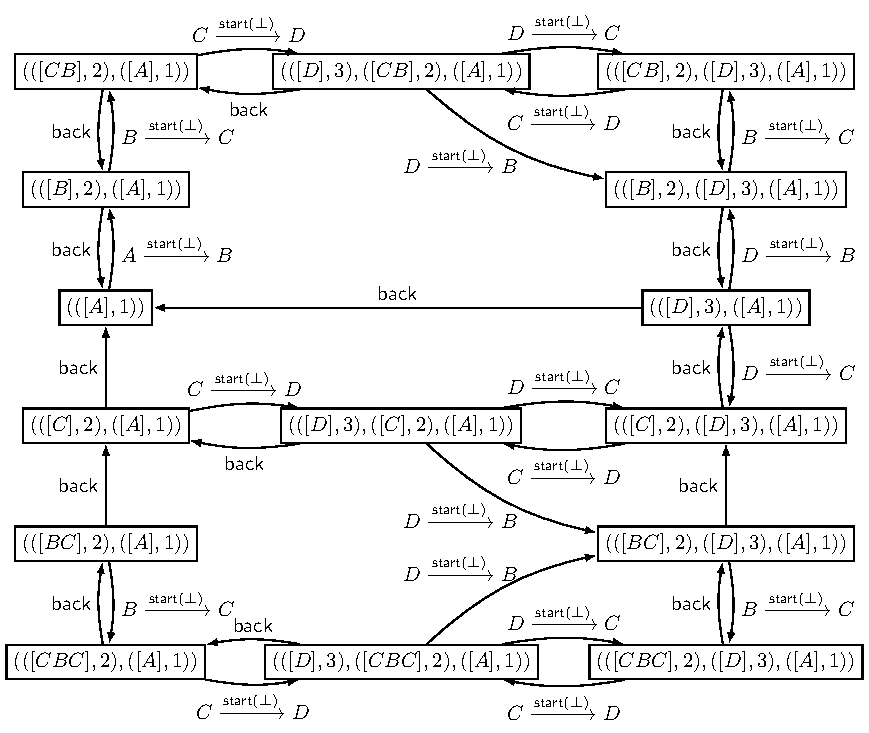
\includegraphics[scale = 0.75]{lmasm-example.pdf}
			\caption{Configurations reachable from the initial configuration $(([A], 1))$ in the $\LMAMASS$ $\Mm$}
				%in $\phi$
		% \vspace{-6mm}	
		\label{lmasm-example}
	\end{figure}
\end{example}

% Intuitively, $\STD$ is similar to $\STP$, without considering the case where $\lmd(A) = \SIT$, when a $\STD$ activity $B$ is started, it is directly pushed into the top task. 
% Recall that $\STP$ is shorthand of SingleToP, when a $\STP$ activity $B$ is started, it is pushed into the top task if the top activity of the top task is \emph{not} $B$.

% $\SIT$ is similar to $\STK$, for each $\SIT$ (resp. $\STK$) activity $B$, it can appear at most once in the configuration. However, they still have differences. Recall that $\SIT$ is shorthand for SingleInsTance, that means the task which $\SIT$ activity located has only one activity. This also explains why starting an $\STD$ or $\STP$ activity, it is \emph{not} pushed into the current task when the callee activity is an $\SIT$ activity.
% Moreover, when starting an activity $B$, if $\lmd(B)\in\{\STK,\SIT\}$ or the callee activity is the $\SIT$ activity, the first step is to specify to which task it will be allocated, more precisely, is to find the task which has the same task affinity with the caller activity. If the task is not found, it will launch a new task $[B]$ on the top of the configuration, if such a task $S_i$ is found, then $S_i$ will be moved to the top task of the configuration, and
% \begin{itemize}
% 	\item if $\lmd(B) = \STD$, then it will directly pushed into $S_i$,
% 	\item if $\lmd(B) = \STP$, it is pushed into $S_i$ if the top activity of $S_i$ is \emph{not} $B$.
% 	\item if $\lmd(B) = \SIT$, then $S_i$ will not change,
% 	\item if $\lmd(B) = \STK$, then it will directly pushed into $S_i$ when $B\notin S_i$, it will poped until the top activity is $B$ otherwise,
% \end{itemize}

\subsection{Semantics of $\IFAMASS$}
% In this case, we only consider the intent flags.
%To define the semantics of $\IFAMASS$, we add some auxiliary functions and predicates. 


%To define the semantics of $\IFAMASS$, we adapt slightly the notion of configurations and the auxiliary functions and predicates. 

Let $\Mm$ be an $\IFAMASS$, namely, $\lmd(A) = \STD$ and $\aft(A) = \aft(A_0)$ for each activity $A$. As a result, there is only one task in each configuration and the task allocation mechanism can be ignored here. Therefore, a configuration here is simply a word $[A_1,\cdots,A_m]\in\act^+$. 
% there is only one task in $\IFAMASS$.

Before formally defining the semantics of $\Mm$, let us first describe the intuitions of the intent flags. 
We would like to warn that although the intuitions of these intent flags may help the readers to get some preliminary idea of their meanings, before diving directly into the formal semantics, they are nonetheless inaccurate, especially when different flags may interfere with each other.

\paragraph{Intuitions of the Intent flags.}  Let us explain the intuitions of the five intent flags in the sequel. 
\begin{itemize}
	\item The $\stpflag$ intent flag:  If it is set,  it has the same effect as starting an activity of the $\STP$ launch mode.
	\item The $\ctpflag$ intent flag:  If it is set, it will check for the existence of the started activity in the task. If the activity exists, then all the activities above the topmost occurrence of the started activity in the task will be removed. Otherwise, the started activity will be pushed into the task.
	\item The $\rtfflag$ intent flag:  If it is set, it will check for the existence of the started activity in the task. If the activity exists, then the topmost occurrence of this activity will be moved to the top of this task. Otherwise, the started activity will be pushed into the task.
	\item The $\ntkflag$ intent flag:  If it is set, it will look for an existing task to put the started activity according to the task allocation mechanism. If such a task exists, the task will be moved to the top and the started activity is pushed to the task, otherwise a new task is created to put this activity.
	\item The $\ctkflag$ intent flag:  It is usually used together with $\ntkflag$. If it is set, it will remove all the activities in the task and push the started activity to the task.
\end{itemize}
%Moreover, $\ntkflag$ will only affect $\ctkflag$ in $\IFAMASS$, since there is only one task in $\IFAMASS$, task allocation mechanism will always allocate the top task.

%To define the semantics of $\IFAMASS$, the concept of configuration is adapted from the definition of configuration for $\LMAMASS$ as follows: A configuration of $\Mm$ is encoded as $[A_1,\cdots,A_m]\in\act^+$.

%Then we introduce some additional and adapted auxiliary functions and predicates that are to be used in the formal semantics of $\IFAMASS$.\\
Moreover, we introduce some additional functions and predicates. 
%\emph{Auxiliary functions and predicates.} 
Let $\rho$ be a configuration with $\rho = [A_1,\cdots,A_m]$. Then
%We define the following auxiliary functions and predicates.
\begin{itemize}
	% \item $\topact(\rho) = A_1$, $\btmact(\rho) = A_m$,
%	\item $\push(\rho, B) = [B, A_1,\cdots,A_m]$,
%	\item $\Pop(\rho) = [A_2,\cdots,A_m]$,
	% \item $\mvacttop(\rho, B) = ([B]\cdot S_1'\cdot S_1'', S_2, \cdots, S_n)$, if $S_1=S_1'\cdot[B]\cdot S_1''$ with $S_1'\in (\act\setminus\{B\})^*$,
%	\item $\clrtop(\rho, B) = [A_j,\cdots,A_m]$, if $A_j = B$ for some $j\in[m]$ and $B\notin[A_1,\cdots,A_{j-1}]$,
	\item $\mvacttop(\rho, B) = [A_j,A_1,\cdots,A_{j-1},A_{j+1},\cdots A_m]$, if $A_j = B$ for some $j\in[m]$ and $B\notin[A_1,\cdots,A_{j-1}]$,
	\item $\clrtsk(\rho, B) = [B]$.
\end{itemize}
Intuitively $\mvacttop(\rho, B)$ is used for defining the semantics of $\rtfflag$, and $\clrtsk(\rho, B)$ is used for defining the semantics of $\ctkflag$.

We are ready to define the semantics of $\IFAMASS$, that is, the relation $\rho \xrightarrow[\Mm]{\tau} \rho'$.
Let $\rho = [A_1,\cdots,A_m]$ for some $m\ge 1$ be the current configuration and $A_1 = A$. 

If $\tau = \back$ then $\rho' = \pop(\rho)$.

Let us assume  $\tau = A\xrightarrow[]{\startactivity(\phi)}B$ in the sequel.

\begin{itemize}
    \item If $\phi\models\ctkflag\wedge\ntkflag$, then $\rho' = \clrtsk(\rho, B)$.
    \item Otherwise,
    \begin{itemize}
        \item if $\phi \models\ctpflag$ and $B \in \rho$, then $\rho' =\clrtop(\rho, B)$,
		\item otherwise,
		\begin{itemize}
			\item if $\phi \models \rtfflag$ and $B \in \rho$, then $\rho'=\mvacttop(\rho, B)$,
			\item otherwise,
			\begin{itemize}
				\item if $\phi \models \stpflag$ and $A = B$, then $\rho' = \rho$,
				\item otherwise, $\rho' = \push(\rho, B)$.
			\end{itemize}
		\end{itemize}
    \end{itemize}
\end{itemize}
Let us use the following example to illustrate the semantics.
\begin{example}
	Let $\Mm = (\act,A,\lmd,\aft,\Delta)$ be an $\IFAMASS$, where $\act = \{A,B,C,D\}$, where for each $A'\in\act$, $\lmd(A') = \STD$ and $\aft(A') = 1$. 
	Moreover, $\Delta = \{\tau_1, \tau_2, \tau_3, \tau_4, \tau_5, \tau_6\}$, where 
		% $\rho_0 = (([D_1],D_1,1))$, and\
			$\tau_1 = A \xrightarrow{\startactivity(\ctkflag)} B$,
			$\tau_2 = B \xrightarrow{\startactivity(\rtfflag)} C$,
			$\tau_3 = C \xrightarrow{\startactivity(\ctpflag)} B$,
			$\tau_4 = C \xrightarrow{\startactivity(\rtfflag)} B$,
			$\tau_5 = C \xrightarrow{\startactivity(\ntkflag\wedge\ctkflag)} D$,
			$\tau_6 = D \xrightarrow{\startactivity(\stpflag)} D$.
	Then the configurations that are reachable from the initial configuration $[A]$ by executing the transition rules from $\Delta$ are illustrated in Figure~\ref{ifasm-example}, where the vertices denote the configurations and the edges denote the elements of $\xrightarrow[\Mm]{}$. 
	For instance, 
	\begin{itemize}
	\item if $A \xrightarrow{\startactivity(\ctkflag)} B$ is applied to the configuration $[A]$, then $B$ is pushed, since $\phi\models\neg\ntkflag \wedge \neg \ctpflag \wedge \neg \rtfflag \wedge \neg \stpflag$, resulting to the configuration $[BA]$,
	%
	\item if $B \xrightarrow{\startactivity(\rtfflag)} C$ is applied to the configuration $[BA]$, then $C$ is pushed, since $\phi\models\rtfflag$ and $C$ does not occur in the task $[BA]$, resulting to the configuration $[CBA]$,
	%
	\item if $C \xrightarrow{\startactivity(\ctpflag)} B$ is applied to the configuration $[CBA]$, then all the activities above $B$, which is $C$ here, are removed from the task, since $\phi\models\ctpflag$ and $B$ occurs in the task $[CBA]$, resulting to the configuration $[BA]$,
	%
	\item if $C \xrightarrow{\startactivity(\rtfflag)} B$ is applied to the configuration $[CBA]$, then $B$ is moved to the top of the task, since $\phi\models\rtfflag$ and $B$ occurs in the task $[CBA]$, resulting to the configuration $[BCA]$,
	%
	\item if $B \xrightarrow{\startactivity(\rtfflag)} C$ is applied to the configuration $[BCA]$, then $C$ is moved to the top of the task, since $\phi\models\rtfflag$ and $C$ occurs in the task $[BCA]$, resulting to the configuration $[CBA]$,
	%
	\item if $C \xrightarrow{\startactivity(\ntkflag\wedge\ctkflag)} D$ is applied to the configuration $[CBA]$, then all activities are removed from the task and $D$ is pushed, since $\phi\models\ntkflag\wedge\ctkflag$, resulting to the configuration $[D]$,
	%
	\item if $D \xrightarrow{\startactivity(\stpflag)} D$ is applied to the configuration $[D]$, then $D$ is not pushed, since $\phi\models\stpflag$ and $D$ is the top activity of the task, resulting to the configuration $[D]$.
	\end{itemize}
	Note that for $\Mm$, there are only finitely many configurations reachable from the initial configuration, which may not be the case for $\IFAMASS$ in general.  
		% $(([D_1],D_1,1))$\\
		% $\xrightarrow[\tau_1]{\Mm}(([P_1D_1],D_1,1))$\\
		% $\xrightarrow[\tau_2]{\Mm}(([P_1D_1],D_1,1))$\\
		% $\xrightarrow[\tau_3]{\Mm}(([K_2],K_2,0),([P_1D_1],D_1,1))$\\
		% $\xrightarrow[\tau_4]{\Mm}(([D_1K_2],K_2,0),([P_1D_1],D_1,1))$\\
		% $\xrightarrow[\tau_5]{\Mm}(([T_2],T_2,0),([D_1K_2],K_2,0),([P_1D_1],D_1,1))$\\
		% $\xrightarrow[\tau_6]{\Mm}(([K_2],K_2,0),([T_2],T_2,0),([P_1D_1],D_1,1))$\\
		
	
		
	\begin{figure}
		% \vspace{-3mm}
			\centering
			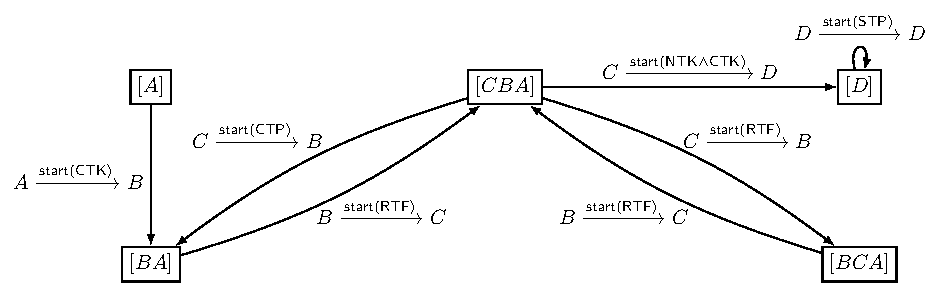
\includegraphics[scale = 0.75]{ifasm-example.pdf}
			\caption{Configurations reachable from the initial configuration $[A]$ in an $\IFAMASS$ $\Mm$}
				%in $\phi$
		% \vspace{-6mm}	
		\label{ifasm-example}
	\end{figure}
\end{example}
% In this case, we assume that the launch modes of activities are $\STD$.  Intuitively, for a transition $A\xrightarrow{\startactivity(\phi)}B$, the intent flags in $\phi$ may depend on each other. The dependency can exhibit in the following two forms: (1) $n$ \emph{subsumes} $n'$, i.e., $n'$ is ignored if $n$ co-occurs with $n'$, and the ``subsume'' relations are transitive, (2) $n$ \emph{enables} $n'$, i.e., $n'$ takes effect if $n$ co-occurs with $n'$. We summarize the dependencies among the intent flags in Figure xxx, 

% For a transition $A\xrightarrow{\startactivity(\phi)}B$, we conclude that :
% \begin{itemize}
% 	\item when $\ctkflag$ tasks effect, then the task will be cleared, and $B$ is pushed into the task,
% 	\item when $\ctpflag$ tasks effect, then the task will be poped until the top activity is $B$ when $B$ is in the task, $B$ will be pushed into the task otherwise, which is similar with the case $\lmd(B) = \STK$,
% 	\item when $\rtfflag$ tasks effect, then $B$ is escalated to the top of the task when $B$ is in the task, $B$ will be pushed into the task otherwise, 
% 	\item when $\stpflag$ tasks effect, then $B$ is pushed into the task when the top activity of the task is not $B$, which is similar with the case $\lmd(B) = \STP$.
% \end{itemize}

\subsection{Semantics of $\AMASS$}
%To define the semantics of $\AMASS$, we use the same definition of configuration as $\LMAMASS$, and add some auxiliary functions and predicates. 

Let $\Mm$ be an $\AMASS$. For clarity, in the sequel, we restate the aforementioned functions $\mvacttop$ and $\clrtsk$ for the configurations that may contain multiple tasks. 
%\emph{Auxiliary functions and predicates.} 
Let $\rho = ((S_1,\aname_1),\cdots, (S_n,\aname_n))$ be a configuration.
Then
\begin{itemize}
	\item $\mvacttop(\rho, B) = (([B]\cdot S_1'\cdot S_1'',\aname_1), (S_2,\aname_2), \cdots, (S_n,\aname_n))$, if $S_1=S_1'\cdot[B]\cdot S_1''$ with $S_1'\in (\act\setminus\{B\})^*$,
	\item $\clrtsk(\rho, B) = (([B],\aname_1), (S_2,\aname_2), \cdots, (S_n,\aname_n))$.
\end{itemize}
% In this case, we consider the launch modes, task affinities and intent flags.
Now we define the semantics of $\AMASS$. 

The semantics of the transition rule $\tau = \back$ is similar to that of $\LMAMASS$.

Let us  assume $\tau = A\xrightarrow[]{\startactivity(\phi)}B$ in the sequel.

Let $\rho = ((S_1,\aname_1),\cdots,(S_n,\aname_n))$ be the current configuration for some $n \ge 1$ and $\topact(\rho) = A$. Moreover, let $S_1 = [A_1',\cdots,A_m']$. Evidently, $A = A_1'$.

\medskip

\noindent \fbox{\fbox{$\lmd(B) = \standard$}}
\begin{itemize}
	\item If $\lmd(A) \neq \singleinstance$ and $\phi \models \neg \ntkflag$, 
	\begin{itemize}
        \item if $\phi \models\ctpflag$ and $B \in \toptsk(\rho)$, then $\rho' =\clrtop(\rho, B)$,
		\item otherwise,
		\begin{itemize}
			\item if $\phi \models \rtfflag$ and $B \in \toptsk(\rho)$, then $\rho'=\mvacttop(\rho, B)$,
			\item otherwise,
			\begin{itemize}
				\item if $\phi \models \stpflag$ and $B = \topact(\rho)$, then $\rho' = \rho$,
				\item otherwise, $\rho' = \push(\rho, B)$.
			\end{itemize}
		\end{itemize}
	\end{itemize}
	%
	\item If $\lmd(A) = \singleinstance$ or $\phi \models \ntkflag$, then
	\begin{itemize}
		\item if $\gettsk(\rho, B) = S_i$ for some $i\in[n]$,
		\begin{itemize}
            \item if $\phi \models\ctkflag$, then $\rho' = \clrtsk(\mvtsktop(\rho, i), B)$,
			\item otherwise, 
			\begin{itemize}
				\item if $\phi \models \ctpflag$ and $B \in S_i$, then 
				$$\rho' =\clrtop(\mvtsktop(\rho, i), B),$$
				\item otherwise,
				\begin{itemize}
					\item if $\phi \models \rtfflag$ and $B \in S_i$, then 
					$$\rho'=\mvacttop(\mvtsktop(\rho, i), B),$$
					\item otherwise,
					\begin{itemize}
						\item if $\phi \models \stpflag$ and $B = \topact(S_i)$, then 
						$$\rho' = \mvtsktop(\rho, i),$$
						\item otherwise, $\rho'=\push(\mvtsktop(\rho, i), B)$,
					\end{itemize}
				\end{itemize}
			\end{itemize}
		\end{itemize}
		\item if $\gettsk(\rho, B) = *$, then $\rho' = \newtsk(\rho, B)$.
	\end{itemize}
\end{itemize}

\noindent \fbox{\fbox{$\lmd(B) = \STP$}}
\begin{itemize}
	\item If $\lmd(A) \neq \singleinstance$ and $\phi \models \neg \ntkflag$, 
	\begin{itemize}
        \item if $\phi \models\ctpflag$ and $B \in \toptsk(\rho)$, then $\rho' =\clrtop(\rho, B)$,
		\item otherwise,
		\begin{itemize}
			\item if $\phi \models \rtfflag$ and $B \in \toptsk(\rho)$, then $\rho'=\mvacttop(\rho, B)$,
			\item otherwise,
			\begin{itemize}
				\item if $B = \topact(\rho)$, then $\rho' = \rho$,
				\item otherwise, $\rho' = \push(\rho, B)$.
			\end{itemize}
		\end{itemize}
	\end{itemize}
	%
	\item If $\lmd(A) = \singleinstance$ or $\phi \models \ntkflag$, then
	\begin{itemize}
		\item if $\gettsk(\rho, B) = S_i$ for some $i\in[n]$,
		\begin{itemize}
            \item if $\phi \models\ctkflag$, then $\rho' = \clrtsk(\mvtsktop(\rho, i), B)$,
			\item otherwise, 
			\begin{itemize}
				\item if $\phi \models\ctpflag$ and $B \in S_i$, then 
				$$\rho' =\clrtop(\mvtsktop(\rho, i), B),$$
				\item otherwise,
				\begin{itemize}
					\item if $\phi \models \rtfflag$ and $B \in S_i$, then 
					$$\rho'=\mvacttop(\mvtsktop(\rho, i), B),$$
					\item otherwise,
					\begin{itemize}
						\item if $B = \topact(S_i)$, then $\rho' = \mvtsktop(\rho, i)$,
						\item otherwise, $\rho'=\push(\mvtsktop(\rho, i), B)$,
					\end{itemize}
				\end{itemize}
			\end{itemize}
		\end{itemize}
		\item if $\gettsk(\rho, B) = *$, then $\rho' = \newtsk(\rho, B)$.
	\end{itemize}
\end{itemize}

\noindent \fbox{\fbox{$\lmd(B) = \STK$}}
\begin{itemize}
	\item If $\gettsk(\rho, B) = S_i$ for some $i\in[n]$,
	\begin{itemize}
		\item if $\phi \models\ctkflag$, then $\rho' = \clrtsk(\mvtsktop(\rho, i), B)$,
		\item otherwise, 
		\begin{itemize}
			\item if $B \notin S_i$, then $\rho' = \push(\mvtsktop(\rho, i), B)$,
			\item if $B \in S_i$, then $\rho' = \clrtop(\mvtsktop(\rho, i), B)$.
		\end{itemize}
	\end{itemize}
	\item If $\gettsk(\rho, B) = *$, then $\rho' = \newtsk(\rho, B)$.
\end{itemize}
\noindent \fbox{\fbox{$\lmd(B) = \SIT$}}
\begin{itemize}
	\item If $\gettsk(\rho, B) = S_i$ for some $i \in [n]$, then $\rho' = \mvtsktop(\rho, i)$,
	\item If $\gettsk(\rho, B) = *$, then $\rho' = \newtsk(\rho, B)$.
\end{itemize}


